\section{Classifier Evaluation}
Wir stellen uns die Frage ob das Model gut genug ist, weshalb wir das Modell genauer evaluieren. Dazu nutzen wir unter anderem eine Confusion Matrix.
\subsection{Confusion Matrix}
\textbf{False Positive:} Der berechnete Wert ist 1 und der wahre Wert ist 0. (Fälschlicherweise richtig)\\
\textbf{False Negative:} Der berechnete Wert ist 0 und der wahre Wert ist 1. (Fälschlicherweise falsch)\\
\textbf{True Negative:} Der berechnete Wert ist 0 und der wahre Wert ebenso. (Korrekt)\\
\textbf{True Positive:} Der berechnete Wert ist 1 und der wahre Wert ebenso. (Korrekt)\\
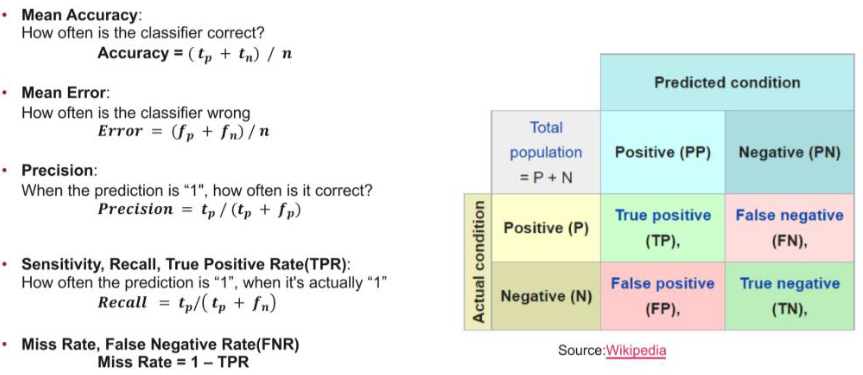
\includegraphics[width=0.8\linewidth]{img/confusion_matrix.png}
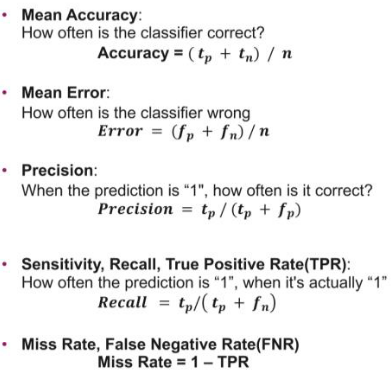
\includegraphics[width=0.8\linewidth]{img/confusion_matrix_description.png}
Bei oben genannten Formeln ist die Mean Accuracy nicht genug um bestimmen zu können, ob wir ein gutes Modell haben. Beispiel: Dataset wo 90\% Nein und 10\% Ja sind. Das Modell sagt nun einfach immer Nein. Hier ist dann die Accurracy bei 90\%. Nun schauen wir die weiteren Werte an Precision und Recall. Diese sind in diesem Modell jeweils 0...
\subsection{Precision vs Recall}
Es kommt drauf an worauf man den Fokus legt je nach Applikation. Nachfolgend die Folie dazu:
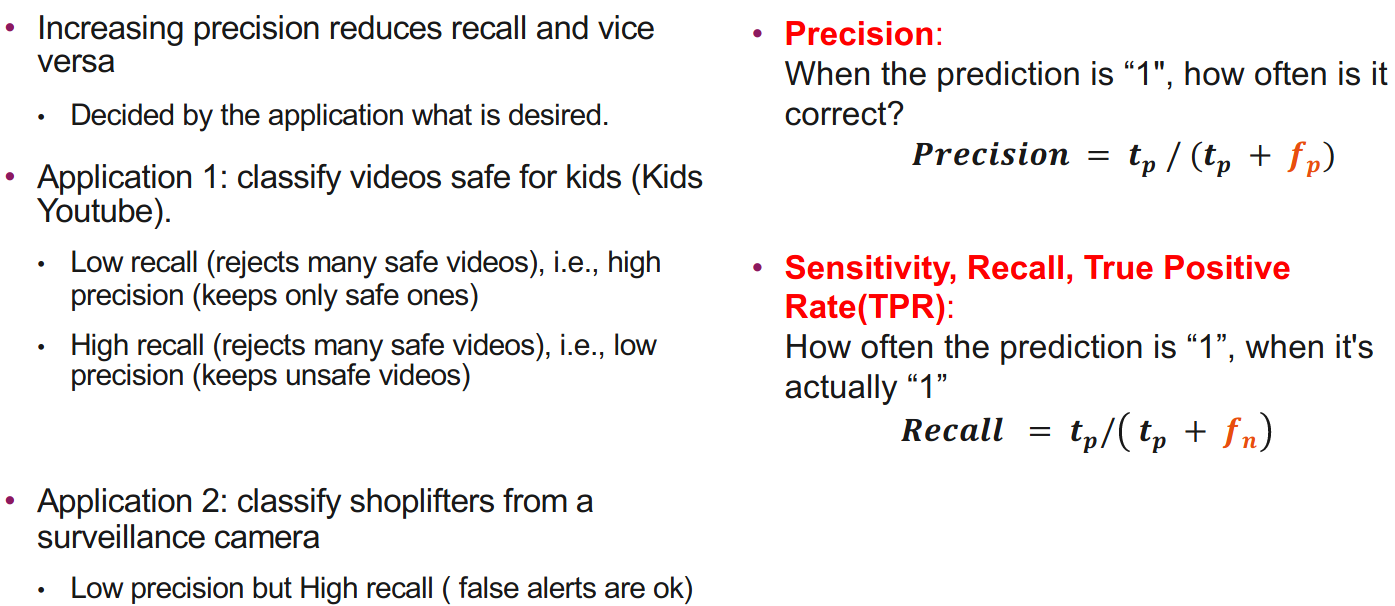
\includegraphics[width=\linewidth]{img/precision_vs_recall.png}
\subsection{Threshold}
Was der Threshold angeht gibt es keine allgemeingültige Lösung mittels Mathematik. Hier kommt es wieder auf die Applikation drauf an. (Threshold ab wann True/False). Vorgehen um das Threshold zu bestimmen:
\begin{enumerate}
\item Modell trainieren
\item Predictions machen mit dem Test-Set
\item Versuchen unterschiedliche Threshold-Werte zu verwenden und damit folgendes berechnen:
\begin{itemize}
\item True Positive Rate (Wie oft richtig akzeptiert) $TPR = t_p/(t_p + f_n)$
\item False Positive Rate (Wie oft falsch akzeptiert) $FPR = f_p/(f_p + t_n)$
\end{itemize}
\item Wir erhalten unterschiedliche TPR und FPR Werte. Diese können wir Plotten -> Ergibt ROC Space (Anderer Plot mit Precision und Recall könnte ein Schnittpunkt ergeben, was sicher ein sehr guter Punkt ist)
\end{enumerate}
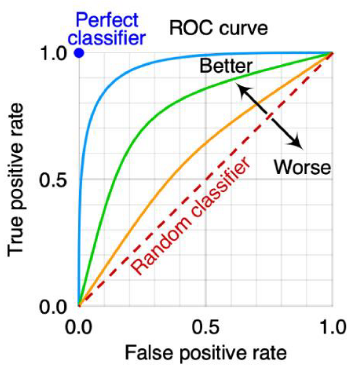
\includegraphics[width=0.6\linewidth]{img/treshold.png}\\
Eine ROC-Kurve ist ein grafisches Diagramm, das die Diagnosefähigkeit eines binären Klassifizierungssystems veranschaulicht, während seine Unterscheidungsschwelle variiert wird. \\
Die ROC-Kurve wird erstellt, indem die Rate der echten positiven Ergebnisse (TPR) gegen die Rate der falschen positiven Ergebnisse (FPR) bei verschiedenen Schwellenwerten aufgetragen wird.
\section{K-Nearest-Neighbours (KNN)}
Haben wir Plots, welche mehr als zwei Klassen haben brauchen wir eine weiter Variante und Logistic Regression wird hier nicht funktionieren. Weiter wird ein lineares Modell nicht zufriedenstellende Ergebnisse Liefern und nicht überall funktionieren:
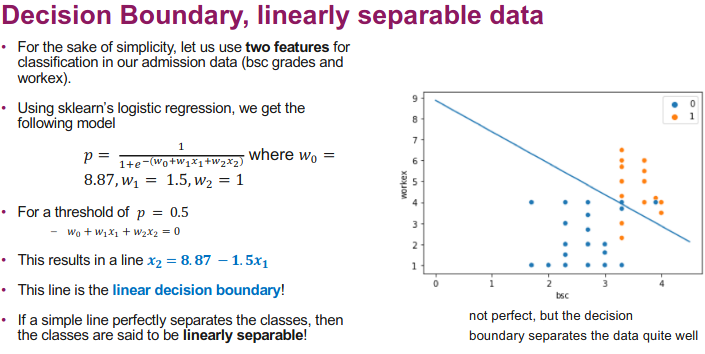
\includegraphics[width=\linewidth]{img/decision_boundary.png}
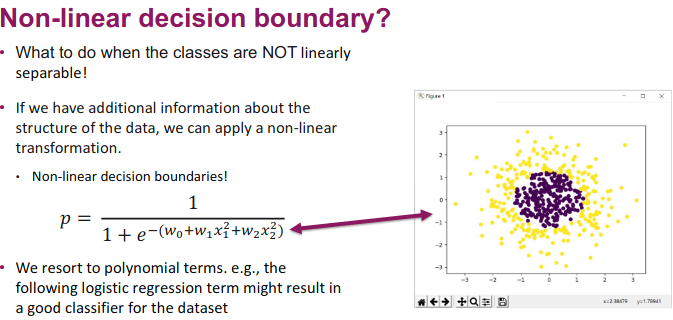
\includegraphics[width=\linewidth]{img/non_linear_decision_boundary.png}
Beispiele für Plots mit mehr als 2 Klassen: SARS-CoV-2 Varianten (Alpha, Beta, Gamma, etc.), Wetter (Sonnig, Wolkig, Regen, Schnee)\\
Logistic Regression kann hier funktionieren, ist aber sehr umständlich. Mann muss viel trainieren (rekursiv), was langsam ist. So braucht es eine Methode ohne training, mit Predictions, einfacher Support mehrere Klassen, und auch möglichkiet Nicht- Lineare-Modelle zu trainieren. Hier kommt KKN ins Spiel.
\subsection{Funktionsweise}
\begin{enumerate}
\item Training und Testdaten laden
\item Value von k bestimmen (Nummer von Nachbaren, welche berücksichtigt werden sollten (1, 5, 10, 15, ...))
\item Für jeden Test-Datenpunkt
\begin{itemize}
\item Für alle Trainingsdaten muss Distanz berechnet werden d(xtest, xtrain): Mit Euclidean, Manhattan, cosine, ...
\item Trainingdaten müssen in ascending Order sortiert werden
\item Die ersten k Datenpunkte werden von der Sortierung genommen
\item Von diesen Punkte werden die am häufigsten vorkommende Klasse genommen als Klassifikation
\end{itemize}
\end{enumerate}
Key-Elemente: Die Anzahl Nachbarn k, Distanz-Metrik\\
\textbf{Beispiel}: Wenn man einen Punkt einer Klasse zuordnen muss und nichts gegeben ist, dann Manhattan Distanz nehmen und um den Punkt ein Quadrat zeichnen, dass  die nächsten N=12 Nachbarn einschliesst und schauen, von welcher Klasse am meisten vorhanden sind.
\subsection{Distanz-Metriken}
Es gibt unterschiedliche Definitionen von Distanzen, die verwendet werden können.
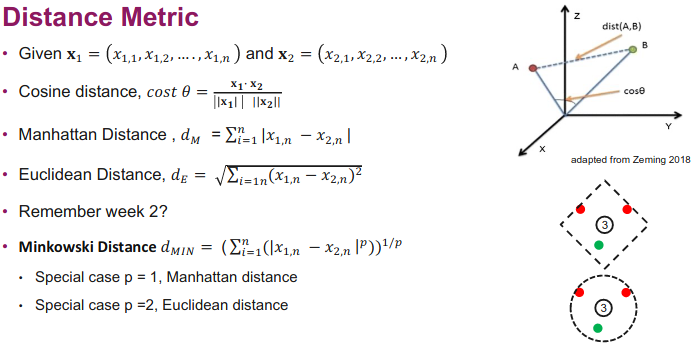
\includegraphics[width=\linewidth]{img/distance_metric.png}
\subsection{Das richtige k und die richtige Distanzmetrik}
Um dies zu bestimmen sollte man folgende Elemente von AI verwenden (Beschrieben in vorangehenden Kapitel):
\begin{itemize}
\item Test-Train split
\item Cross Validation
\item Test Performanceüberwachung (Mean accurarcy, Precision, Recall)
\end{itemize}
\subsection{Vor/Nachteile}
\textcolor{green}{Vorteile:}\\
\begin{itemize}
\item Einfaches Modell
\item Wenige Hyperparameter
\end{itemize}

\textcolor{red}{Nachteile:}
\begin{itemize}
\item K muss gut gewählt werden
\item Grosse Berechnungsaufwand, wenn Sample gross ist
\item Nicht effizient bei vielen Dimensionen
\item Richtige Skalierung muss verfügbar sein
\end{itemize}

\subsection{Beispiel IRIS}
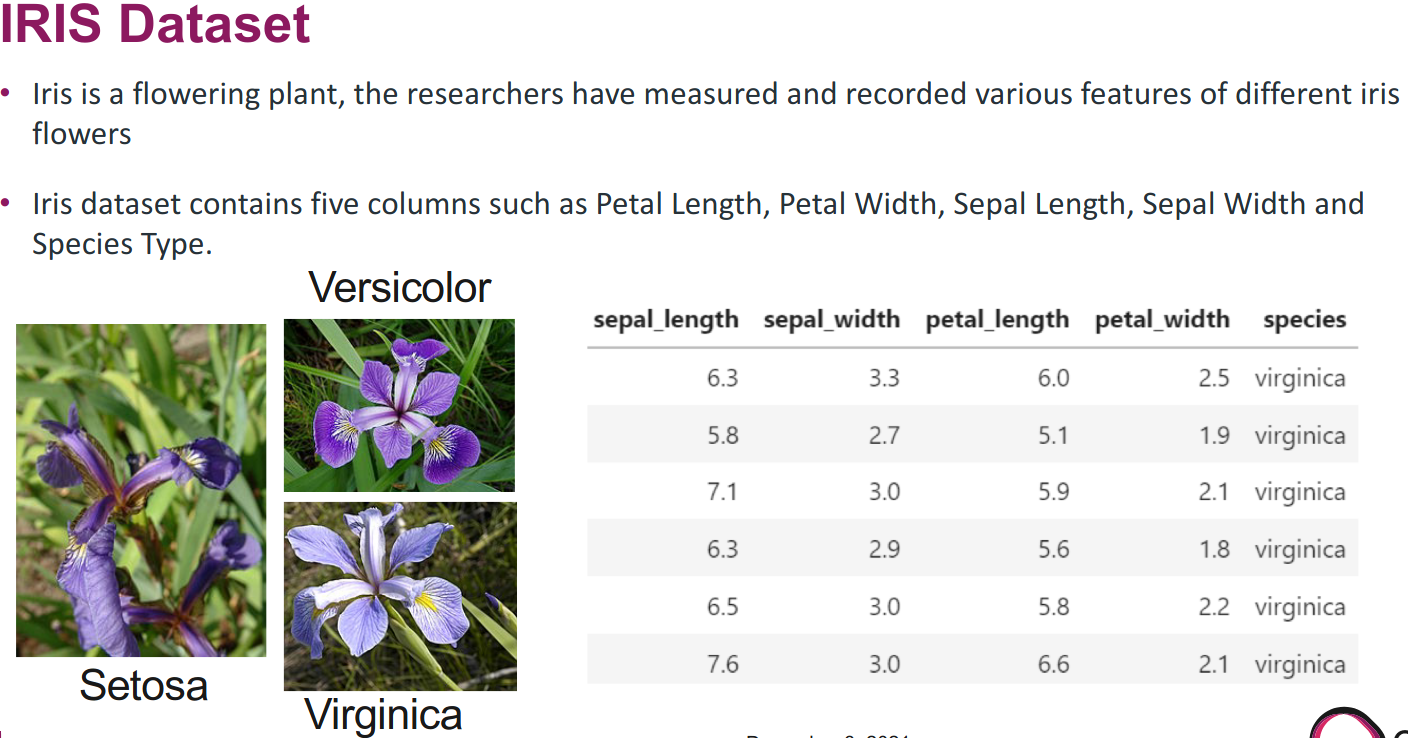
\includegraphics[width=\linewidth]{img/iris.png}